\documentclass[a4paper, 11pt]{article}
\usepackage{textgreek}
\usepackage{caption}
\captionsetup{tablename=Tabella}
\usepackage{slashbox}
\usepackage{pgfplots}
\pgfplotsset{/pgf/number format/use comma,compat=newest}
\usepackage{multirow}
\usepackage{subfigure}

\begin{document}
\section*{Tabelle hash}
\vspace{0,4 cm}
Ci interessa analizzare il comportamento delle tabelle hash al variare del fattore di caricamento $\alpha=n/m$, dove $n$ è il numero di elementi inseriti in tabella e $m$ è la lunghezza di quest'ultima.

\vspace{0,5 cm}
Le tabelle hash sono un'implementazione della struttura dati dizionario. Un dizionario è un insieme di coppie chiave-valore. Tale struttura rende efficiente l'operazione di ricerca (\O$(1)$ per il tempo atteso e $\Theta(n)$ per il tempo nel caso peggiore).\\
Per l'indirizzamento dei dati, cioè la scelta della posizione di un certo oggetto all'interno della tabella, è stato usato il metodo delle divisioni (funzione $h$), il quale inserisce, se la cella è vuota, l'elemento con chiave $k$ nella cella data da $(k)mod(m)$.\\
Per risolvere il problema delle collisioni, cioè quando si vuole inserire un elemento in un posto già occupato, ci sono vari metodi, ma in questo esercizio ne prenderemo in considerazione due:
\begin{itemize}
\item Concatenamento: tutti gli elementi con la stessa chiave sono inseriti a capo della stessa lista, e quindi la tabella hash risulta come una lista che all'interno di ogni cella contiene a sua volta una lista.
\item Indirizzamento aperto con esplorazione lineare: se un elemento trova occupata la cella in cui deve essere inserito, ricalcola la chiave come $(h(k)+i)mod(m)$, dove $i$ è il numero di iterazioni svolte per trovare posto al valore $k$. E' facile intuire che questa esplorazione visita tutte le celle partendo da quella trovata inizialmente in ordine numerico (naturalmente raggiunto il valore $m-1$, se ancora le iterazioni sono minori ad $m$, riparte dalla cella con chiave 0). L'esecuzione si interrompe se trova una cella libera o il numero di iterazioni è uguale ad $m$.
\end{itemize}
Per valutare le prestazioni al variare del fattore di caricamento, si registra il numero di collisioni totali che si ottiene inserendo in una tabella vuota tanti elementi quanti servono per ottenere il fattore di caricamento desiderato.

\vspace{0,5 cm}
Dai test ci si attende che il numero di collisioni sia sempre in crescita all'aumentare del fattore di caricamento. Ci si aspetta inoltre che per il concatenamento il numero di collisioni sia minore rispetto all'indirizzamento aperto. Questo perché, il concatenamento può generare una sola collisione ad elemento inserito, mentre l'indirizzamento aperto, per ogni inserimento, può generare fino a $m$ collisioni. Considerato ciò che è stato appena detto, ci si aspetta che superato il punto in cui fattore di caricamento è 1, cioè dove la tabella è quasi piena per il concatenamento e piena per l' indirizzamento aperto, la crescita delle collisioni risulti costante.

\vspace{0,5 cm}
I test sono stati svolti facendo variare il fattore di caricamento da 0 a 2. Sono state usate tabelle hash con 4 grandezze differenti: 8, 12, 16, 20. Per ogni esecuzioni del test, sono istanziate 4 tabelle (una per ogni grandezza), e inseriti tanti valori quanti servono per portare $\alpha$ a 2. I test sono stati ripetuti 5 volte.

\vspace{0,5 cm}
Seguono i risultati:

\vspace{1 cm}
\begin{table}[h]
\caption{Collisioni con concatenamento}
\hspace{1 cm}
\begin{tabular}{| c | c c c c c c c c |}
\hline
\multicolumn{1}{| c |}{\backslashbox{$m$}{$\alpha$}}& \multicolumn{1}{| c |}{1/4} & \multicolumn{1}{| c |}{1/2} & \multicolumn{1}{| c |}{3/4} & \multicolumn{1}{| c |}{1} & \multicolumn{1}{| c |}{5/4} & \multicolumn{1}{| c |}{3/2} & \multicolumn{1}{| c |}{7/4} & \multicolumn{1}{| c |}{2}\\
\hline
\multirow{5}{*}{8} & 0 & 1 & 1 & 1 & 2 & 4 & 6 & 8\\
& 0 & 1 & 1 & 2 & 3 & 5 & 7 & 9\\
& 0 & 0 & 2 & 4 & 5 & 5 & 7 & 9\\
& 0 & 0 & 2 & 4 & 4 & 6 & 8 & 10\\
& 0 & 1 & 2 & 4 & 6 & 7 & 8 & 10\\
\hline
\multirow{5}{*}{12} & 0 & 2 & 4 & 5 & 5 & 6 & 9 & 12\\
& 0 & 2 & 4 & 5 & 7 & 9 & 11 & 14\\
& 1 & 1 & 2 & 3 & 5 & 8 & 10 & 13\\
& 0 & 0 & 2 & 4 & 7 & 8 & 10 & 12\\
& 0 & 1 & 2 & 3 & 6 & 7 & 9 & 12\\
\hline
\multirow{5}{*}{16} & 0 & 2 & 4 & 7 & 9 & 11 & 14 & 18\\
& 1 & 2 & 3 & 6 & 8 & 12 & 14 & 18\\
& 1 & 3 & 3 & 6 & 8 & 10 & 13 & 17\\
& 0 & 0 & 2 & 4 & 8 & 10 & 13 & 16\\
& 0 & 0 & 3 & 6 & 9 & 11 & 14 & 18\\
\hline
\multirow{5}{*}{20} & 0 & 1 & 2 & 7 & 11 & 14 & 17 & 21\\
& 1 & 1 & 2 & 7 & 12 & 15 & 19 & 22\\
& 0 & 1 & 4 & 7 & 11 & 14 & 19 & 24\\
& 1 & 2 & 5 & 10 & 13 & 17 & 19 & 23\\
& 0 & 2 & 4 & 6 & 9 & 13 & 18 & 22\\
\hline
\end{tabular}
\end{table}
\newpage
\begin{table}[h]
\caption{Collisioni con indirizzamento aperto}
\hspace{1 cm}
\begin{tabular}{| c | c c c c c c c c |}
\hline
\multicolumn{1}{| c |}{\backslashbox{$m$}{$\alpha$}}& \multicolumn{1}{| c |}{1/4} & \multicolumn{1}{| c |}{1/2} & \multicolumn{1}{| c |}{3/4} & \multicolumn{1}{| c |}{1} & \multicolumn{1}{| c |}{5/4} & \multicolumn{1}{| c |}{3/2} & \multicolumn{1}{| c |}{7/4} & \multicolumn{1}{| c |}{2}\\
\hline
\multirow{5}{*}{8} & 0 & 0 & 1 & 9 & 25 & 41 & 57 & 73\\
& 0 & 3 & 7 & 11 & 27 & 43 & 59 & 75\\
& 0 & 0 & 3 & 6 & 22 & 38 & 54 & 70\\
& 1 & 3 & 6 & 9 & 25 & 41 & 57 & 73\\
& 0 & 1 & 1 & 3 & 19 & 35 & 51 & 67\\
\hline
\multirow{5}{*}{12} & 0 & 1 & 3 & 22 & 58 & 94 & 130 & 166\\
& 0 & 3 & 6 & 20 & 56 & 92 & 128 & 164\\
& 1 & 1 & 1 & 8 & 44 & 80 & 116 & 152\\
& 0 & 1 & 5 & 21 & 57 & 93 & 129 & 165\\
& 0 & 0 & 1 & 19 & 55 & 91 & 127 & 163\\
\hline
\multirow{5}{*}{16} & 0 & 5 & 23 & 34 & 98 & 162 & 226 & 290\\
& 0 & 3 & 7 & 29 & 93 & 157 & 221 & 285\\
& 0 & 0 & 6 & 37 & 101 & 165 & 229 & 293\\
& 1 & 5 & 9 & 30 & 94 & 158 & 222 & 286\\
& 1 & 1 & 6 & 37 & 101 & 165 & 229 & 293\\
\hline
\multirow{5}{*}{20} & 0 & 0 & 3 & 29 & 129 & 229 & 329 & 429\\
& 0 & 3 & 14 & 61 & 161 & 261 & 361 & 461\\
& 0 & 4 & 12 & 45 & 145 & 245 & 345 & 445\\
& 2 & 6 & 15 & 55 & 155 & 255 & 355 & 455\\
& 0 & 1 & 11 & 46 & 146 & 246 & 346 & 446\\
\hline
\end{tabular}
\end{table}
\begin{figure}[h]
\caption{Numero collisioni al crescere di $\alpha$}
\footnotesize
\centering
\hspace{-5,5 cm}
\subfigure[Concatenamento]
{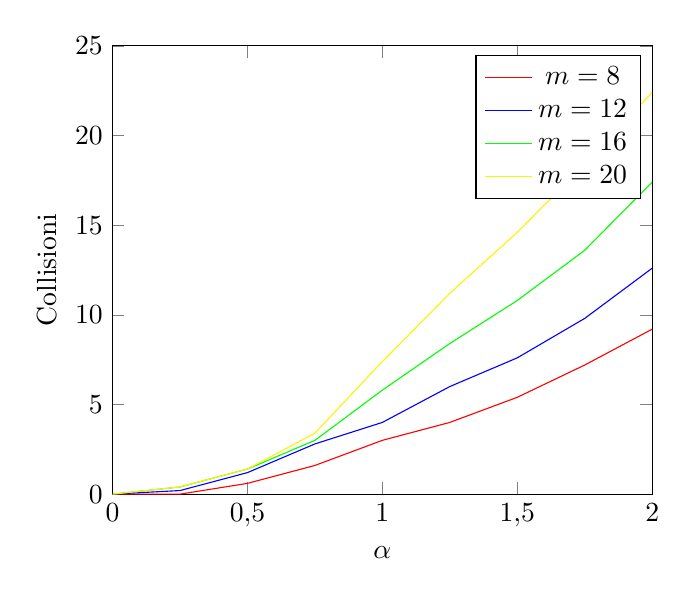
\begin{tikzpicture}
\begin{axis}[xmin=0, xmax=2, ymin=0,ymax=25, xlabel=$\alpha$, ylabel=Collisioni]
\addplot[red]
coordinates{(0,0) (0.25,0) (0.5,0.6) (0.75,1.6) (1,3) (1.25,4) (1.5,5.4) (1.75,7.2) (2,9.2)};
\addplot[blue]
coordinates{(0,0) (0.25,0.2) (0.5,1.2) (0.75,2.8) (1,4) (1.25,6) (1.5,7.6) (1.75,9.8) (2,12.6)};
\addplot[green]
coordinates{(0,0) (0.25,0.4) (0.5,1.4) (0.75,3) (1,5.8) (1.25,8.4) (1.5,10.8) (1.75,13.6) (2,17.4)};
\addplot[yellow]
coordinates{(0,0) (0.25,0.4) (0.5,1.4) (0.75,3.4) (1,7.4) (1.25,11.2) (1.5,14.6) (1.75,18.4) (2,22.4)};
\legend{$m=8$,$m=12$,$m=16$,$m=20$}
\end{axis}
\end{tikzpicture}}
\hspace{1 cm}
\subfigure[Indirizzamento aperto]
{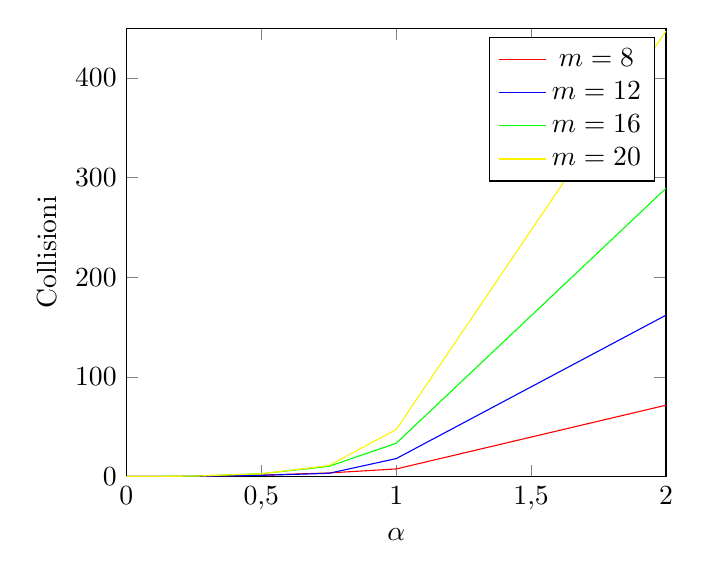
\begin{tikzpicture}
\begin{axis}[xmin=0, xmax=2, ymin=0,ymax=450, xlabel=$\alpha$, ylabel=Collisioni]
\addplot[red]
coordinates{(0,0) (0.25,0.2) (0.5,1.4) (0.75,3.6) (1,7.6) (1.25,23.6) (1.5,39.6) (1.75,55.6) (2,71.6)};
\addplot[blue]
coordinates{(0,0) (0.25,0.2) (0.5,1.2) (0.75,3.2) (1,18) (1.25,54) (1.5,90) (1.75,126) (2,162)};
\addplot[green]
coordinates{(0,0) (0.25,0.4) (0.5,2.8) (0.75,10.2) (1,33.4) (1.25,97.4) (1.5,161.4) (1.75,225.4) (2,289.4)};
\addplot[yellow]
coordinates{(0,0) (0.25,0.4) (0.5,2.8) (0.75,11) (1,47.2) (1.25,147.2) (1.5,247.2) (1.75,347.2) (2,447.2)};
\legend{$m=8$,$m=12$,$m=16$,$m=20$}
\end{axis}
\end{tikzpicture}}
\hspace{-5 cm}
\vspace{-4,5 cm}
\end{figure}
\newpage
I risultati confermano che superato il valore 1 per il fattore di caricamento, la crescita delle collisioni assume un andamento lineare.\\
Proprio per il fatto che il caso di concatenamento genera al massimo una sola collisione, mentre l'indirizzamento aperto ne può generare fino ad $m$, il numero di collisioni nel secondo caso risulta molto più grande, così come il coefficiente della retta da cui il grafico assume l'andamento.\\
Naturalmente al crescere di $m$ cresce anche il numero di collisioni calcolate nei test. Questo è dato dal fatto che più $m$ è grande, maggiore è il numero di elementi da inserire nella tabella per far crescere $\alpha$.

\vspace{1 cm}
\textbf{Documentazione codice}

\vspace{0,7 cm}
Il programma è stato scritto con Python nell'ambiente di sviluppo Pycharm.

\vspace{0,5 cm}
Per la realizzazione abbiamo usato due classi:
\begin{itemize}
\item \emph{Element}: istanzia oggetti con una chiave che possono contenere altri dati al loro interno. Essendo questo un esercizio destinato solo a capire il funzionamento delle tabelle hash, non sono mai inseriti dei dati all'interno dell'elemento.
\item \emph{HashTable}: istanzia una tabella hash grande quanto indicato nel valore \emph{hash\textunderscore{length}} in ingresso al costruttore. La tabella è a concatenamento se \emph{hash\textunderscore{type}} in ingresso al costruttore è uguale a 0, se invece il valore è uguale ad 1 allora la tabella è a indirizzamento aperto. 
\end{itemize}
Inoltre è presente il metodo \emph{division\textunderscore{method}} esterno alle classi. Questo metodo calcola la chiave corrispondente ad un elemento all'interno di una tabella hash ($h(k)$) data la chiave dell'elemento ($k$) e la lunghezza della tabella ($m$).

\vspace{0,5 cm}
I test descritti sopra sono riportati nel \emph{main} del file.
\end{document}